\documentclass[11p, titlepage, oneside, a4paper]{article}
% Packages
\usepackage{amsmath}
\usepackage{graphicx}
\usepackage{hyperref}
\usepackage[english,swedish]{babel}
\usepackage[
    backend=biber,
    style=authoryear-ibid,
    sorting=ynt
]{biblatex}
\usepackage[utf8]{inputenc}
\usepackage[T1]{fontenc}
\usepackage{booktabs}
%Källor
\addbibresource{mall.bib}
\graphicspath{ {./images/} }

% Ändra de rader som beh 1över ändras
\def\inst{Teknikprogrammet}
\def\typeofdoc{Laborationsrapport}
\def\course{Fysik 1 150p}
\def\pretitle{Laboration 1}
\def\title{Rörelse: Hastighet och acceleration}
\def\name{Henrik Forsberg}
\def\username{henrik.forsberg}
\def\email{\username{}@elev.ga.ntig.se}
\def\graders{Magnus Silverdal}

\begin{document}

\begin{titlepage}
		\thispagestyle{empty}
		\begin{large}
			\begin{tabular}{@{}p{\textwidth}@{}}
				\textbf{NTI gymnasiet \hfill \today} \\
				\textbf{\inst} \\
				\textbf{\typeofdoc} \\
			\end{tabular}
		\end{large}
		\vspace{10mm}
		\begin{center}
			\LARGE{\pretitle} \\
			\huge{\textbf{\course}}\\
			\vspace{10mm}
			\LARGE{\title} \\
			\vspace{15mm}
			\begin{large}
				\begin{tabular}{ll}
					\textbf{Namn} & \name \\
					\textbf{E-mail} & \texttt{\email} \\
				\end{tabular}
			\end{large}
			\vfill
            
\includegraphics[width=0.5\textwidth]{images/NTI Gymnasiet_Symbol_print_svart.png}
			\vfill
            \large{\textbf{Handledare}}\\
			\mbox{\large{\graders}}
		\end{center}
	\end{titlepage}

    \begin{otherlanguage}{english}
	\begin{abstract}
        This is the ``sammanfattning'', it is written in english and called the abstract.      
    \end{abstract}
    \end{otherlanguage}
    % Om arbetet är långt har det en innehållsförteckning, annars kan den utelämnas
	\pagenumbering{roman}
	\tableofcontents
	
	% och lägger in en sidbrytning
	\newpage

	\pagenumbering{arabic}
	
	% i Sverige har vi normalt inget indrag vid nytt stycke
	\setlength{\parindent}{0pt}
	% men däremot lite mellanrum
	\setlength{\parskip}{10pt}
	
	\section{Syfte och frågeställning}
		Syftet med labborationen var att ta reda på en bils hastighet och acceleration under en rörelse längst efter en bana.

	\section{Bakgrund och teori}
	    Programmet kan utifrån en film använda sig av motiontracking och mäta hur långt ett föremål har rört sig under en viss tid. Sedan använder jag denna data för och räknar ut medelacceleration $a_m = \frac{\Delta v}{\Delta t}$ och medelhastighet $v_m = \frac{\Delta s}{\Delta t}$ i excel vilket ger en en graf som visar både medelacceleration och en som visar medelhastighet. Om tidsstegen är tillräckligt korta så blir medelvärdet ungefär lika med momentanvärdet och i filmen så finns det 60 stycken i sekunden vilket är tillräckligt för att det skulle bli tillräckligt nära.

	\section{Metod och materiel}
        \begin{enumerate}
            \item Vagn
            \item Lutande plan med ställning
            \item Linjal
            \item Mobilkamera
        \end{enumerate}
        
        Det lutande planet ställs på ena änden på en dator och en laddare på det lägre bordet längst fram i Arkimedes och andra änden på det högre bordet, se figur \ref{fig:lutandeplan}. Kameran placeras vid sidan av uppställningen på ett avstånd så att hela rörelsen ryms i filmen utan att kameran behöver flyttas. Vagnen rullas nedför planet samtidigt som kameran filmar rörelsen. Försöket placeras så att ljusförhållanden och bakgrund ger en så tydlig och skarp film som möjligt.
        
        \begin{figure}[!h]
            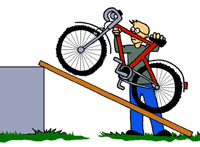
\includegraphics[width=0.8\textwidth]{images/lutandePlan.jpg}
            \caption{En blid hade varit superbra här}
            \label{fig:lutandeplan}
        \end{figure}
        
        Filmen analyserades sedan med mjukvaran Tracker för att få fram en tabell med positionen som funktion av tiden.
    \newpage
	\section{Analys och beräkning}
        Datat från analysen av filmen visas i tabell \ref{table:result}
    

        \begin{table}
            \centering
            \begin{tabular}{ll}
                \toprule
                \textbf{Tid (s)} & \textbf{Position (m)} \\
                \midrule
                3,33E-02 & 1,18E+01 \\
                6,64E-02 & 1,12E+01 \\
                6,65E-02 & 1,10E+01 \\
                9,97E-02 & 1,23E+01 \\
                9,98E-02 & 1,40E+01 \\
                1,33E-01 & 1,53E+01 \\
                1,33E-01 & 1,94E+01 \\
                1,66E-01 & 2,07E+01 \\
                1,66E-01 & 2,21E+01 \\
                1,99E-01 & 2,18E+01 \\
                1,99E-01 & 2,64E+01 \\
                2,33E-01 & 2,18E+01 \\
                2,33E-01 & 6,567532 \\
                2,66E-01 & -6,697113 \\
                2,66E-01 & -2,911043 \\
                2,99E-01 & -3,831482 \\
                2,99E-01 & -2,99E+01 \\
                3,32E-01 & 4,65E+01 \\
                3,32E-01 & 5,39E+01 \\
                3,65E-01 & 3,64E+01 \\
                3,66E-01 & 4,78E+01 \\
                3,99E-01 & 5,34E+01 \\
                3,99E-01 & 4,10E+01 \\
                4,32E-01 & 5,19E+01 \\
                4,32E-01 & 3,86E+01 \\
                4,65E-01 & 5,00E+01 \\
                4,65E-01 & 5,03E+01 \\
                4,98E-01 & 5,43E+01 \\
                4,98E-01 & 7,10E+01 \\
                5,32E-01 & 8,73E+01 \\
                5,32E-01 & 1,03E+02 \\
                5,65E-01 & 1,21E+02 \\
                5,65E-01 & 1,41E+02 \\
                5,98E-01 & 1,57E+02 \\
                5,98E-01 & 1,75E+02 \\
                6,31E-01 & 1,94E+02 \\
                6,31E-01 & 2,12E+02 \\
                6,64E-01 & 2,32E+02 \\
                6,65E-01 & 2,51E+02 \\
                6,98E-01 & 2,76E+02 \\
                6,98E-01 & 2,94E+02 \\
                7,31E-01 & 3,22E+02 \\
                7,31E-01 & 3,41E+02 \\
                7,64E-01 & 3,61E+02 \\
                7,64E-01 & 3,85E+02 \\
                7,97E-01 & 4,16E+02 \\
                7,97E-01 & 4,45E+02 \\
                8,14E-01 & 4,65E+02 \\
                8,47E-01 & 4,89E+02 \\
                8,47E-01 & 5,09E+02 \\
                8,80E-01 & 5,34E+02 \\
                8,80E-01 & 5,62E+02 \\
                9,14E-01 & 5,74E+02 \\
                9,14E-01 & 6,15E+02 \\
                9,47E-01 & 6,26E+02 \\
                9,47E-01 & 5,55E+02 \\
                9,80E-01 & 6,75E+02 \\
                9,80E-01 & 7,01E+02 \\
                1,01E+00 & 6,58E+02 \\
                1,01E+00 & 7,49E+02 \\
                \bottomrule
            \end{tabular}
            \caption{Mätväden}
            \label{table:result}
        \end{table}


    Datat importeras i Excel och hastigheten beräknas med hjälp av formeln $v_m = \frac{\Delta s}{\Delta t}$ och acceleration med formeln $a_m = \frac{\Delta v}{\Delta t}$.
    
    \section{Slutsats och resultat} 
        Resultatet av beräkningarna illustreras i graferna 1 och 2.

        \begin{figure}[!h]
            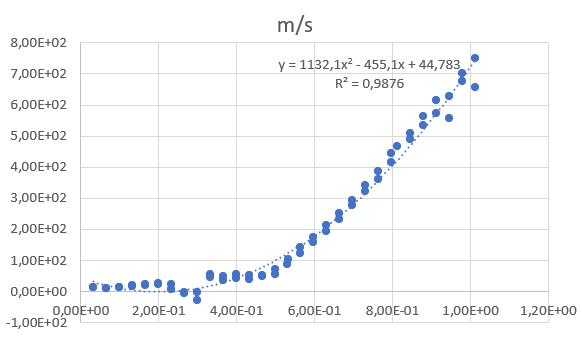
\includegraphics[width=0.8\textwidth]{images/graph 1.png}
            \caption{Sträcka/Tid diagram}
            \label{fig:Graf 1}
        \end{figure}

        \begin{figure}[!h]
            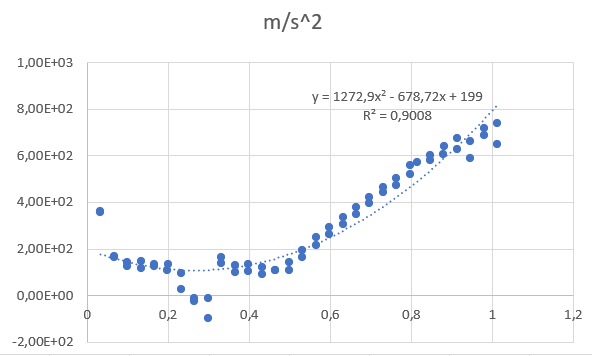
\includegraphics[width=0.8\textwidth]{images/graph 2.png}
            \caption{Acceleration/Tid diagram}
            \label{fig:Graf 2}
        \end{figure}

        Här kan man tydligt se att hastigheten ökar kvadratiskt eftersom att det är en x^2 funktion på trendlinjen i Graf 1. Accelerationen var också kvadratiskt ökande som man kan se i Graf 2. Jag var dock tvungen att ta bort den första punkten vilket är varför den första punkten inte börjar på t = 0. Detta var eftersom att det blev ett väldigt tydligt mätfel som förstörde graferna.

    \section{Diskussion} 
    Resultaten blev fel vilket man kan se eftersom att hastighetendiagramets trendlinje inte har R = 1 vilket den teoretiskt skulle ha. Detta är eftersom att kameran vi använde inte var perfekt och eftersom att bilen som användes var tillräckligt stor så programmet läste av olika delar av bilen vid olika bilder av filmen.
    
    \printbibliography

\end{document}

